%version of 10-22-19

\chapter{$\oplus$ Additional Material on the Fibonacci Numbers}
\label{ch:FIBO-enrich}

\section{$\oplus$ Computations on the Fibonacci Numbers}
\label{sec:FIBO-enrich-ops}

\index{The Fibonacci Quartlerly}
One reason that the Fibonacci sequence has captivated an entire mathematically oriented community are the myriad identities involving Fibonacci numbers, which are simply presented and gracefully verified.\footnote{An entire research journal, {\it The Fibonacci Quarterly}, is dedicated to the mathematics of recursively defined sequences of numbers---the genre epitomized by the Fibonacci numbers.}  This section is dedicated to two particularly beautiful,  unintuitive, identities.

\subsection{$\oplus$ Products of Consecutive Fibonacci Numbers}
\label{sec:product-Fn-Fn+1}
\index{Fibonacci numbers!product of consecutive}

Our first identity asserts the equality of each product $F(n) \cdot F(n-1)$ of two consecutive Fibonacci numbers, with the sum of the squares of the first $n$ Fibonacci numbers.

\begin{prop} 
\label{thm:FiboSumConsecutive}
For all $n \geq 1$,
\begin{equation}
\label{eq:FiboSumConsecutive}
F(n) \cdot F(n-1) \ \ = \ \ \sum_{k=0}^{n-1} (F(k))^2.
\end{equation}
\end{prop}

\begin{proof}
One can observe identity (\ref{eq:FiboSumConsecutive}) ``in action''
in Fig.~\ref{fig:fibosquare}.  We augment this visual validation of
the identity with the following induction.

\medskip

\noindent {\it Base case.}
Instance $n=1$ of identity (\ref{eq:FiboSumConsecutive}) is valid
because
\[ F(0) \cdot F(1) \ = \ 1 \cdot 1 \ = \ 1^2 \ = \ (F(0))^2. \]

\medskip

\noindent {\it Inductive hypothesis.}
Assume that identity (\ref{eq:FiboSumConsecutive}) is valid for all $n
\leq m$.

\medskip

\noindent {\it Inductive extension.}
Let us focus on the product $F(m+1) \cdot F(m)$.  Invoking the defining Fibonacci recurrence
(\ref{eq:Fibonacci-defn}) and the inductive hypothesis, we generate the following chain of identities.
\begin{eqnarray*}
F(m+1) \cdot F(m)
 & = &
   (F(m) \ + \ F(m-1)) \cdot F(m) \\
 & = &
   (F(m))^2 \ \ + \ \ F(m) \cdot F(m-1)  \\
 & = & 
   (F(m))^2  \ \ + \ \ \sum_{k=0}^{m-1} (F(k))^2  \\
 & = &
   \sum_{k=0}^{m} (F(k))^2.
\end{eqnarray*}
The induction is thus extended, which completes the proof.
\qed
\end{proof}



\subsection{$\oplus \oplus$ Greatest Common Divisors of Fibonacci Numbers}
\label{Appendix:FiboGCD}

Our second identity exposes the marvelous fact that the {\em greatest common divisor} ({\sc gcd}) of an arbitrary pair of Fibonacci numbers is again a Fibonacci number!

\begin{prop}
For all integers $m, n, \in \N$,
\begin{equation}
\label{eq:fibo-gcd}
\mbox{\sc gcd} \left(F(m), F(n) \right) \ = \ F \left(\mbox{\sc gcd}(m, n) \right).
\end{equation}
\end{prop}

\medskip

\noindent
To make identity (\ref{eq:fibo-gcd}) at least plausible, we cite a single example:

\hspace*{.35in}
$\mbox{\sc gcd}(F(12), F(18)) 
   \ = \ \mbox{\sc gcd}(144,2584)
   \ = \ 8 \ = \ F(6)$,

\noindent while

\hspace*{.35in}
$\mbox{\sc gcd}(12,18) \ = \ 6$.

\medskip

\begin{proof}
Let us assume, with no loss of generality,  that $n \geq m$.  Our proof proceeds by verifying, in turn, the following divisibilities:
\begin{enumerate}
\item
$\mbox{\sc gcd}(n,m)$ divides $\mbox{\sc gcd}(F(n), F(m))$

\item
$\mbox{\sc gcd}(F(n), F(m))$ divides $\mbox{\sc gcd}(n,m)$
\end{enumerate}

\smallskip

\noindent
We leave to the reader the exercise of verifying the following three technical lemmas.

{\Arny Verifying these lemmas is exactly what I would define as an EXERCISE}

\begin{lemma}
\label{lem:FIBO-GCD-1}
The following relation holds for any integers $n$ and $k \geq 1$:
\[  F(n+k) \ = \ F(k) \cdot F(n+1) \ + \ F(k-1) \cdot F(n) \] 
\end{lemma}

\noindent
The proof is a straightforward induction on $k$ for fixed $n$.

%\footnote{this relation assumes that we are able to define negative Fibonacci numbers.  Well, there is a "natural" way of extending the definition to negative numbers...}

\begin{lemma}
\label{lem:FIBO-GCD-2}
For any integer $k$, $F(n)$ divides $F(k \cdot n)$.
\end{lemma}

\noindent
This lemma can be obtained from Lemma~\ref{lem:FIBO-GCD-1}.

\begin{lemma}
\label{lem:FIBO-GCD-3}
If integer $a$ divides integer $b$, then $F(a)$ divides $F(b)$.
\end{lemma}

\medskip

\noindent
We are able now to verify identity (\ref{eq:fibo-gcd}) via the following assertions.

\medskip

\begin{enumerate}
\item
{\em $F(\mbox{\sc gcd}(n,m))$ divides $\mbox{\sc gcd}(F(n), F(m))$.}

\smallskip

By definition of ``{\sc gcd}", $\mbox{\sc gcd}(n,m)$ divides both $n$ and $m$.  Because of this,
Lemma~\ref{lem:FIBO-GCD-3} guarantees that $F(\mbox{\sc gcd}(n,m))$ divides both $F(n)$ and $F(m)$, hence, divides their {\sc gcd}.

\medskip

\item
{\em $\mbox{\sc gcd}(F(n), F(m))$ divides $F(\mbox{\sc gcd}(n,m))$.}

\smallskip

$\mbox{\sc gcd}(n,m)$ can be written as a linear combination, $a n + b m$, of $n$ and $m$.  (In fact, it is the smallest such combination.). Therefore, 
\[ F(\mbox{\sc gcd}(n,m)) \ = \ F(a n + b m) \]
for some integers $a$ and $b$.  Lemma~\ref{lem:FIBO-GCD-1} assures us, then, that
$F(\mbox{\sc gcd}(n,m))$ is a multiple of $n$ and, symmetrically, of $m$; therefore, it is a multiple of their {\sc gcd}. 
\end{enumerate}
This completes the proof.   \qed
\end{proof}


\section{$\oplus \oplus$ A Number System Based on the Fibonacci Sequence}
\label{sec:numerals-special-families}
\label{sec:Fibo-numbers}

\subsection{Preliminaries}
\label{sec:FIBO-num-intro}

This section continues our mathematical-cultural tour of the Fibonacci numbers, the recursively defined sequence of numbers which has been of considerable significance for centuries.  Our study of the sequence until now, in Sections~\ref{sec:Fibonacci} and~\ref{sec:FIBO-enrich-ops}, has focused ``inward", deriving results that are important for understanding the sequence.  In contrast, we focus on the ``outward"-looking application of the sequence.

History has lent us many examples of nonstandard representations of the integers proving significant for reasons that go far beyond the representation of numbers.  We have repeatedly benefited from such unexpected uses of number representations, which arise from the ability of mathematical objects to ``encode" a broad range of situations.  (Two simple examples: ($a$) the use of base-$2$ numerals to count in various combinatorial applications; ($b$) the use of prime-power representations within the realm of coding.)  This section is devoted to developing a system for representing integers, which is based on the family of Fibonacci numbers.

\subsection{Zeckendorf's Theorem}
\label{sec:Zeckendorf's-Theorem}

\index{Zeckendorf, Edouard}

The endeavor of using Fibonacci numbers to represent arbitrary integers is based on the following theorem by the Belgian mathematician Edouard Zeckendorf \cite{Zeckendorf72}.

\smallskip

To simplify exposition, we employ two nonstandard conventions in what follows.
\begin{enumerate}
\item
{\em We index the Fibonacci sequence starting at index $1$, not the traditional $0$.}
\item
{\em For integers $m$ and $n$, we write ``$m \gg n$" to mean that $m \geq n+2$.}
\end{enumerate}

\begin{prop}[Zeckendorf's Theorem]
\label{thm:Zeckendorf}
Every positive integer $n$ has a unique representation as the sum of nonconsecutive Fibonacci numbers with indices $k \geq 2$.  In detail, this representation has the form

\smallskip

\hspace*{.25in} $n \ = \ F(k_1) \ + \ F(k_2) \ + \cdots + \ F(k_\ell)$

\smallskip

\noindent
where \ \ $k_1 \ \gg \ k_2 \ \gg \cdots \gg \ k_\ell \ \geq \ 2$.
\end{prop}

\medskip

We remark that the injunction against employing $F(1)$ in a representation is no real restriction because under our nonstandard convention for the indices of Fibonacci numbers, $F(1)=F(2)$.

\medskip

\index{Zeckendorf representation}

Call a representation of an integer $n$ a {\it Zeckendorf representation} if it satisfies the conditions of Proposition~\ref{thm:Zeckendorf}.

\medskip

\noindent {\it Illustrating the Zeckendorf representation.}

\noindent $\bullet$
The Zeckendorf representation of the integer $12345$ is:
\[ \begin{array}{ccccccccccc}
12345 & =  & 10946 & + & 987    & +  &   377  & + & 34   & + & 1 \\
           & =  & F(21)  & + & F(16)  & +  & F(14) & + & F(9) & + & F(2)
\end{array} \]     

\medskip

\noindent $\bullet$
Fig.~\ref{fig:zeckendorf} illustrates the Zeckendorf representations of the first $26$ integers. 
\begin{figure}[h]
\begin{center}
%\includegraphics[width=0.4\textwidth]{../FIGmaths/zeckendorf_representations.png}
        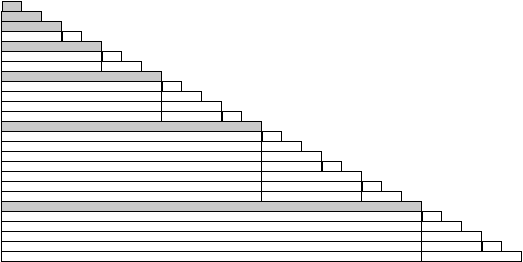
\includegraphics[scale=0.5]{FiguresArithmetic/Zeckendorf}
        \caption{The first $26$ integers (on the vertical [Y] axis), represented in the Zeckendorf system.  The breaks in the horizontal bars represent the summations of Fibonacci numbers.  The shaded horizontal bars correspond to pure Fibonacci numbers.}
\label{fig:zeckendorf}
\end{center}
\end{figure}

\subsection{A Proof of Zeckendorf's Theorem}
\label{sec:Zeckendorf-proof}

Our proof accomplishes three goals simultaneously:
\begin{itemize}
\item
It specifies an algorithm for constructing a Zeckendorf representation of every argument integer $n$.
\item
It verifies that the resulting representation is
  \begin{itemize}
  \item
{\em valid}---the Fibonacci numbers that it uses in the representation do, indeed, sum to $n$
  \item
{\em unique}---no other selection of Fibonacci numbers that satisfy Proposition~\ref{thm:Zeckendorf} yields numbers that sum to $n$.
  \end{itemize}
\end{itemize}
A single induction on $n$ accomplishes all three goals.  Keep in mind our nonstandard indexing of the Fibonacci sequence.

\smallskip

\noindent {\sf Base cases}.
The base of the induction is the case $n=2$.  To wit, $F(3) = 2$, and no other sum of Fibonacci numbers that satisfy Proposition~\ref{thm:Zeckendorf} yield the value $n=2$.

Similarly, Proposition~\ref{thm:Zeckendorf} holds for the cases $n=3$ and $n=4$ also.  To wit, $F(4) = 3$, and $F(4) + F(2) = 3 + 1 = 4$; uniqueness is left as an exercise.

\smallskip

\noindent {\sf Inductive hypothesis}.
Assume for induction that any integer $m < F(r)$ admits a unique representation of the form specified in Proposition~\ref{thm:Zeckendorf}.

\smallskip

\noindent {\sf Inductive extension}.
Focus on an arbitrary integer $n$ in the interval
\[ [F(r) \leq n < F(r+1)] \]
We claim that every $n$ in this interval admits a unique Zeckendorf representation.

Of course, this claim is true for the smallest $n$ in the interval, namely, $n=F(r)$, because the equation ``$n=F(r)$" obviously specifies a valid Zeckendorf representation of $n$.  (We leave it to the reader to verify that this representation is unique.)

Focus, therefore, for an arbitrary $n \neq F(r)$ within the interval.  Write this $n$ in the form $n = F(r) + m$.  Note that we must have $m < F(r)$, by specification of the interval and by the defining recurrence of the Fibonacci sequence.  Consequently, our inductive hypothesis tells us that the integer $m$ admits a unique Zeckendorf representation:

\hspace*{.25in} $m \ = \ F(k_1) \ + \ F(k_2) \ + \cdots + \ F(k_\ell)$

\smallskip

\noindent
where \ \ $k_1 \ \gg \ k_2 \ \gg \cdots \gg \ k_\ell \ \geq \ 2$.

\noindent
This means that the integer $n$ admits a representation of the form

\hspace*{.25in} $n \ = \ F(r) \ + \ F(k_1) \ + \ F(k_2) \ + \cdots + \ F(k_\ell)$

\smallskip

\noindent
where \ \ $k_1 \ \gg \ k_2 \ \gg \cdots \gg \ k_\ell \ \geq \ 2$.

\smallskip 

Our final task is to verify that $F(r)$ and $F(k_1)$ are not consecutive Fibonacci numbers, or equivalently, to verify that $F(k) \gg F(k_1)$.  To this end, assume, for contradiction, that $k_1=r-1$.  Were this the case, we would have (from the Fibonacci recurrence)
\[ n \ = \ F(r+1) \ + \ F(k_2) \ + \cdots + \ F(k_\ell) \]
which would contradict the fact that $n < F(r+1)$.  This argument verifies the uniqueness as well as the validity of $n$'s Zeckendorf representation.

**HERE
\subsection{Applications of the Fibonacci number system}

Any unique system of representation is a numbering system.

The previous theorem ensures that any non-negative integer can be written
as a sequence of bits $b_i$, in other words,

$n = (b_mb_{m-1}...b_2)_F$ iff $n = \Sigma_{k=2}^m b_k F(k)$.

Note: we wrote here the representation of $n$ in the Fibonacci numbering system using parenthesis in order to avoid confusions 
on the indices.

Let us compare this system to the binary representation.
For instance, the Fibonacci representation of $12345$ is $100001010000100000010_F$
while  $12345 = 2^{13} + 2^{12} + 2^{5} + 2^{4} + 2^{3} + 2^{0} = 1100000111001_2$.
The binary representation is more compact. 
\bigskip

The decomposition in the Fibonacci basis of the first integers (starting from $1 = 00001_F$) is as follows:

 $2 = 0010_2 = F(3) = 00010_F$
 
 $3 = 0011_2 = F(4) = 00100_F$
  
 $4 = 100_2 = 3+1 = 00101_F$
 
 $5 = 101_2 = F(5) = 01000_F$
 
 $6 = 110_2 = 5+1 = 01001_F$
 
 $7 = 111_2 = 5+2 = 01010_F$
 
 $8 = 1000_2 = F(6) = 10000_F$
 
 $9 = 1001_2 = 10001_F$
 
 $10 = 1010_2 = 10010_F$
 
 $11 = 1011_2 = 10100_F$
 
 $12 = 1100_2 = 10101_F$
 
 $13 = 1101_2 = F(7) = 100000_F$
 
 ...
 
There is no consecutive digits equal to $1$ in such representations.
\medskip

{\Denis I can write briefly how to perform an addition within this system, what do you think?}
{\Arny Definitely yes}

